\documentclass[12pt]{article}

\usepackage{sbc-template}
\usepackage{graphicx,url}
\usepackage{algorithm}
\usepackage{algpseudocode} 
\usepackage[utf8]{inputenc}  

     
\sloppy

\title{Relatório 2 da Implementação de Projeto e Análise de Algoritmos}

\author{Camila Lopes\inst{1}, Victor Colen\inst{1} }


\address{Instituto de CIências Exatas e Informática \\ Pontifícia Universidade Catórila de Minas Gerais (PUC-MG)\\
  30535-901 -- Coração Eucarístico -- Belo Horizonte – MG - Brasil
  \email{\{lopes.camila, victor.costa\}@sga.pucminas.br}
}

\begin{document} 

\maketitle

\begin{resumo} 
 Este artigo apresenta três algoritmos para busca de elementos em um vetor de inteiros, sendo eles: busca linear, busca binária e busca linear com o uso de sentinela. Ademais, é realizada uma comparação entre os métodos com base no número de operações necessárias para localizar um elemento específico no vetor. 
\end{resumo}


\section{Introdução}
A busca eficiente de elementos em estruturas de dados é um problema fundamental na ciência da computação e no desenvolvimento de algoritmos, com aplicações em diversas áreas. Dessa forma, neste artigo projetamos três algoritmos para busca em vetores de inteiros: busca linear, busca binária e busca linear com sentinela. 

A busca linear é o método mais simples, percorrendo sequencialmente o vetor até encontrar o elemento desejado. A busca binária, por sua vez, aproveita-se de vetores ordenados para reduzir drasticamente o espaço de busca a cada iteração. Já a busca linear com sentinela é uma variação otimizada da busca linear que elimina a necessidade de verificar o fim do vetor a cada iteração.

Posto isto, neste estudo, comparamos esses três algoritmos em termos do número de operações necessárias para encontrar um elemento específico, em quatro cenários diferentes: um cenário com o elemento no começo do vetor, no meio do vetor, no final do vetor e um cenário onde o elemento não está presentes no vetor. Dessa forma, nossa análise considera as distribuições de elementos, proporcionando uma visão abrangente da eficiência relativa de cada método.

\section{Implementação}

\subsection{Busca Linear}
A implementação da busca linear é direta e simples, o algoritmo percorre sequencialmente o vetor, comparando cada elemento com o valor buscado. Dessa forma, retorna verdadeiro se encontrado ou um indicador de falha caso contrário. Esta abordagem tem complexidade de tempo \textbf{O(n)} no pior caso, onde n é o número de elementos no vetor.

\begin{algorithm}
    \caption{Algoritmo de Busca Linear}
    \label{alg:estruturaDeDados_GD}
    \begin{algorithmic}
        \State \textbf{Entrada:} Array $array$, tamanho do array $n$, elemento $x$
        \State operações $\gets 0$
        \For{$i = 0$ até $n-1$}
            \State operações $\gets$ operações $+ 1$
            \If{$array[i] = x$}
                \State operações $\gets$ operações $+ 1$
                \State \textbf{retorna} Verdadeiro, operações
            \EndIf
            \State operações $\gets$ operações $+ 1$
        \EndFor
        \State operações $\gets$ operações $+ 1$
        \State \textbf{retorna} Falso, operações
    \end{algorithmic}
\end{algorithm}

\newpage
\subsection{Busca Binária}
A implementação da busca binária requer um vetor previamente ordenado. Dessa forma, o algoritmo começa comparando o elemento buscado com o elemento central do vetor. Se forem iguais, a busca é concluída, caso contrário, é descartado metade do vetor baseado na comparação e repete o processo na metade restante. Assim, este processo continua, reduzindo pela metade o espaço de busca a cada iteração, até encontrar o elemento ou determinar que ele não existe no vetor. 

A complexidade de tempo deste algoritmo é \textbf{O(log n)}, tornando-o eficiente para grandes conjuntos de dados ordenados.

\begin{algorithm}
    \caption{Algoritmo de Busca Binária}
    \label{alg:estruturaDeDados_GD}
    \begin{algorithmic}
         \State \textbf{Entrada:} Array $array$, índices $left$ e $right$, elemento $x$
        \State operações $\gets 0$
        \While{$left \leq right$}
            \State operações $\gets$ operações $+ 1$
            \State $mid \gets left + (right - left) / 2$
            \State operações $\gets$ operações $+ 4$
            \If{$array[mid] = x$}
                \State operações $\gets$ operações $+ 1$
                \State \textbf{retorna} Verdadeiro, operações
            \ElsIf{$array[mid] < x$}
                \State $left \gets mid + 1$
                \State operações $\gets$ operações $+ 2$
            \Else
                \State $right \gets mid - 1$
                \State operações $\gets$ operações $+ 2$
            \EndIf
        \EndWhile
        \State operações $\gets$ operações $+ 1$
        \State \textbf{retorna} Falso, operações
    \end{algorithmic}
\end{algorithm}

\subsection{Busca Linear com Sentinela}
A implementação da busca linear com sentinela é considerado uma otimização da busca linear tradicional. Neste algoritmo, antes de iniciar a busca, o valor procurado é temporariamente adicionado ao final do vetor como uma 'sentinela', dessa forma, é eliminado a necessidade de verificar o fim do vetor a cada iteração, simplificando o loop de busca. Assim, após percorrer o vetor, é verificado se o elemento encontrado está na posição da sentinela (indicando que o elemento não estava originalmente no vetor) ou em uma posição anterior (indicando sucesso na busca). 

Embora mantenha a complexidade \textbf{O(n)} no pior caso, esta técnica pode oferecer uma melhoria de desempenho na prática, especialmente para vetores grandes.

\begin{algorithm}
    \caption{Algoritmo de Busca Linear com Sentinela}
    \label{alg:estruturaDeDados_GD}
    \begin{algorithmic}
        \State \textbf{Entrada:} Array $array$, índice do último elemento $lastIndex$, elemento $x$
        \State operações $\gets 0$
        \State $array[lastIndex] \gets x$
        \State operações $\gets$ operações $+ 2$
        \State $i \gets 0$
        \State operações $\gets$ operações $+ 1$
        \While{$array[i] \neq x$}
            \State $i \gets i + 1$
            \State operações $\gets$ operações $+ 2$
        \EndWhile
        \State operações $\gets$ operações $+ 1$
        \State \textbf{retorna} (i $\neq lastIndex$), operações
    \end{algorithmic}
\end{algorithm}

\section{Resultados}

Nesta seção, são apresentados os gráficos que comparam o número de operações necessárias para encontrar um elemento em um vetor de inteiros usando os três algoritmos implementados.

\begin{figure}[!h]
    \centering
    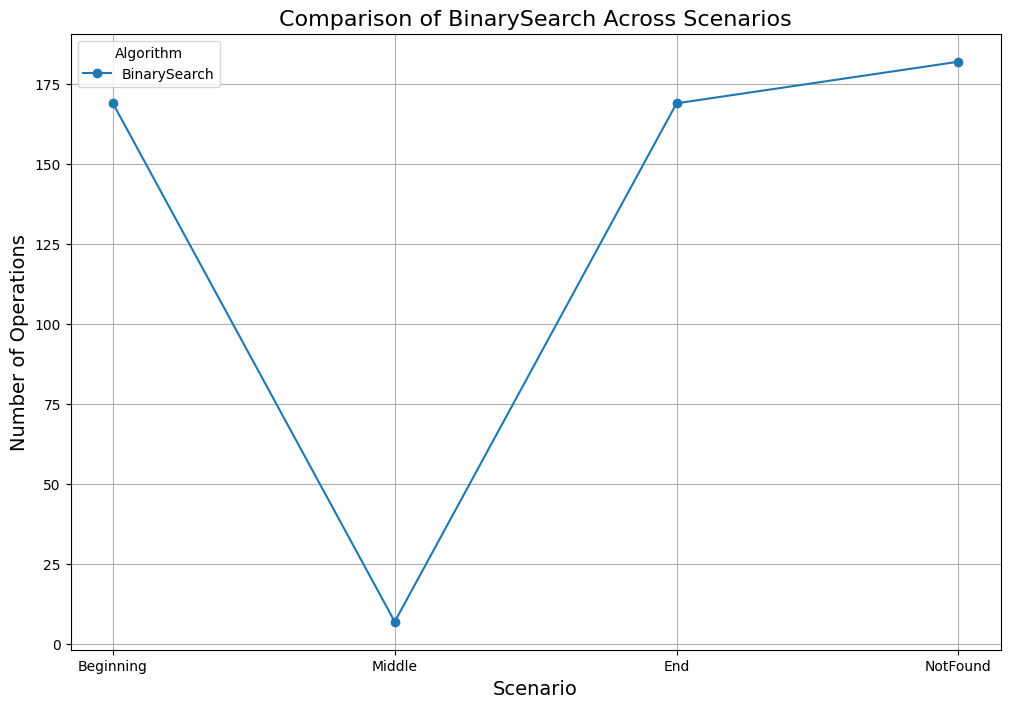
\includegraphics[width=0.8\textwidth]{binary_search_comparison_plot.png}
    \caption{Comparação de operações da busca binária em diferentes cenários.}
    \label{fig:binary-comparison}
\end{figure}

\begin{figure}[!h]
    \centering
    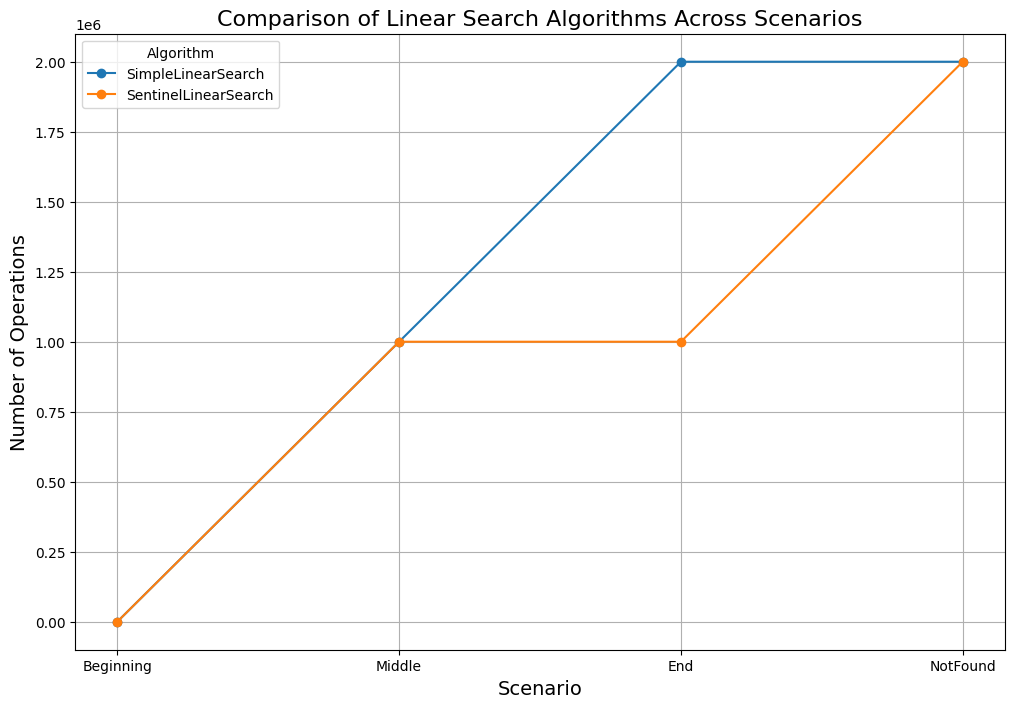
\includegraphics[width=0.8\textwidth]{linear_search_comparison_plot.png}
    \caption{Comparação de operações das buscas lineares (simples e com sentinela) em diferentes cenários.}
    \label{fig:linear-comparison}
\end{figure}

\newpage
Ao comparar os três algoritmos em diferentes cenários, foi possível observar variações significativas no número de operações necessárias. Dessa forma, foi observado que para elementos no início do vetor, a busca linear e a busca linear com sentinela apresentaram um desempenho superior. No caso de elementos no meio, a busca binária demonstrou ser mais eficiente devido à sua complexidade logarítmica. Já para elementos no final do vetor, a busca linear com sentinela demonstrou sua eficiência, sendo superior à busca binária, algo fora da expectativa.

Quando o elemento não está presente, a busca binária demonstrou uma menor quantidade de operações, enquanto a busca linear simples e a busca linear com sentinela deve apresentar o maior número de operações neste último cenário. É importante notar que, embora a busca binária seja geralmente mais eficiente, ela requer um vetor previamente ordenado, o que deve ser considerado na análise global de eficiência.


\section{Conclusão}

Este estudo comparou três algoritmos de busca - busca linear, busca binária e busca linear com sentinela - em um vetor de 100.000 elementos, analisando seu desempenho em diferentes cenários.

A busca binária, como esperado, mostrou-se mais eficiente em cenários com elementos no meio do vetor ou ausentes, especialmente em grandes conjuntos de dados. No entanto, sua necessidade de um vetor pré-ordenado deve ser considerada no cálculo do custo total da operação.

Surpreendentemente, a busca linear com sentinela demonstrou uma melhoria de desempenho em relação à busca linear simples apenas quando o elemento buscado estava no final do vetor. Nos outros cenários, incluindo quando o elemento não estava presente, a diferença de desempenho entre estes dois algoritmos foi insignificante.

A busca binária permanece como a opção mais eficiente para vetores ordenados, especialmente em cenários onde múltiplas buscas são realizadas no mesmo conjunto de dados. Para vetores não ordenados ou em situações onde a ordenação prévia é impraticável, a escolha entre busca linear e busca linear com sentinela deve ser cuidadosamente considerada com base nas características específicas do problema e na distribuição esperada dos dados.

Em conclusão, este estudo reafirma a importância da escolha adequada do algoritmo de busca baseada no contexto específico da aplicação, considerando fatores como o tamanho do conjunto de dados, a frequência das buscas e a possibilidade de manter os dados ordenados. Futuros estudos poderiam explorar o desempenho em cenários mais específicos ou adicionar mais algoritmos para comparação.

%\bibliographystyle{sbc}
%\bibliography{sbc-template}

\end{document}
